\documentclass[english,serif,mathserif]{beamer}
\usetheme[formal,deutsch]{s3it}

\usepackage[T1]{fontenc}
\usepackage[latin9]{inputenc}
\usepackage{babel}

\begin{document}

%% Optional Argument in [Brackets]: Short Title for Footline
\title[Short Title]{Cinder}
\subtitle{Or: Openstack's Block Storage Service}

\author{Tyanko Aleksiev \texttt{<tyanko.aleksiev@s3it.uzh.ch>}}

\date{\today}

\maketitle

\begin{frame}{Cinder's role inside OpenStack}

Cinder is a service used to provide Virtualized Block Storage Devices to the 
end users of OpenStack without requiring them to have any knowledge of where 
that storage is actually deployed or on what type of device.

\vspace{5mm}

The hypervisor simply provides a standard SCSI volume to the VM, very likely
when a user plug-in a USB stick in his laptop.

\end{frame}

\begin{frame}{Cinder components: \textbf{cinder-api}}

The role of \textit{cinder-api} is to accept and manage API calls to:

\begin{itemize}
\item create, delete and list volumes and snapshots,
\item attach and detach volumes (called by nova).
\end{itemize}

\end{frame}


\begin{frame}{Cinder components: \textbf{cinder-scheduler}}

The role of \textit{cinder-scheduler} is to:
\begin{itemize}
\item manage the cooperation between cinder-api and cinder-volume through the message queue and the DB,
\item examine and choose the back-end which is going to provide the storage capacity requested by the user.
\end{itemize}
Different filters are available as plug-ins.

\end{frame}

\begin{frame}{Cinder components: \textbf{cinder-volume}}

The role of \textit{cinder-volume} is to:
\begin{itemize}
\item handle and execute the requests coming from cinder-scheduler,
\item interact directly with variuos types of storage back-ends.
\end{itemize}

Multiple cinder-volumes instances can be run either on the same node 
providing access to different type of storage back-ends or on multiple 
nodes to increase scalability. 

\end{frame}

\begin{frame}{Cinder components: \textbf{Message queues}}

\textit{Messaging queues} are used for communication between the services.
RabbitMQ is a common implementation choice inside OpenStack.  

\end{frame}

\begin{frame}{Cinder components: \textbf{Database}}

A \textit{Database} is used for storing volume metadata. 
A common implementation choice here is MySQL. 

\end{frame}

\begin{frame}{Cinder components: \textbf{Storage}}

\textit{Storage} is the back-end from where the volumes are actually served. 
Different back-end types are supported:

\begin{itemize}
\item LVM 
\item Ceph,
\item Gluster,
\item NFS,
\item ZFS,
\item Sheepdog,
\item SAN from different vendors (IBM, NetApp...)
\end{itemize} 

\end{frame}

\begin{frame}{Cinder: components interaction 1/3}

\centerline{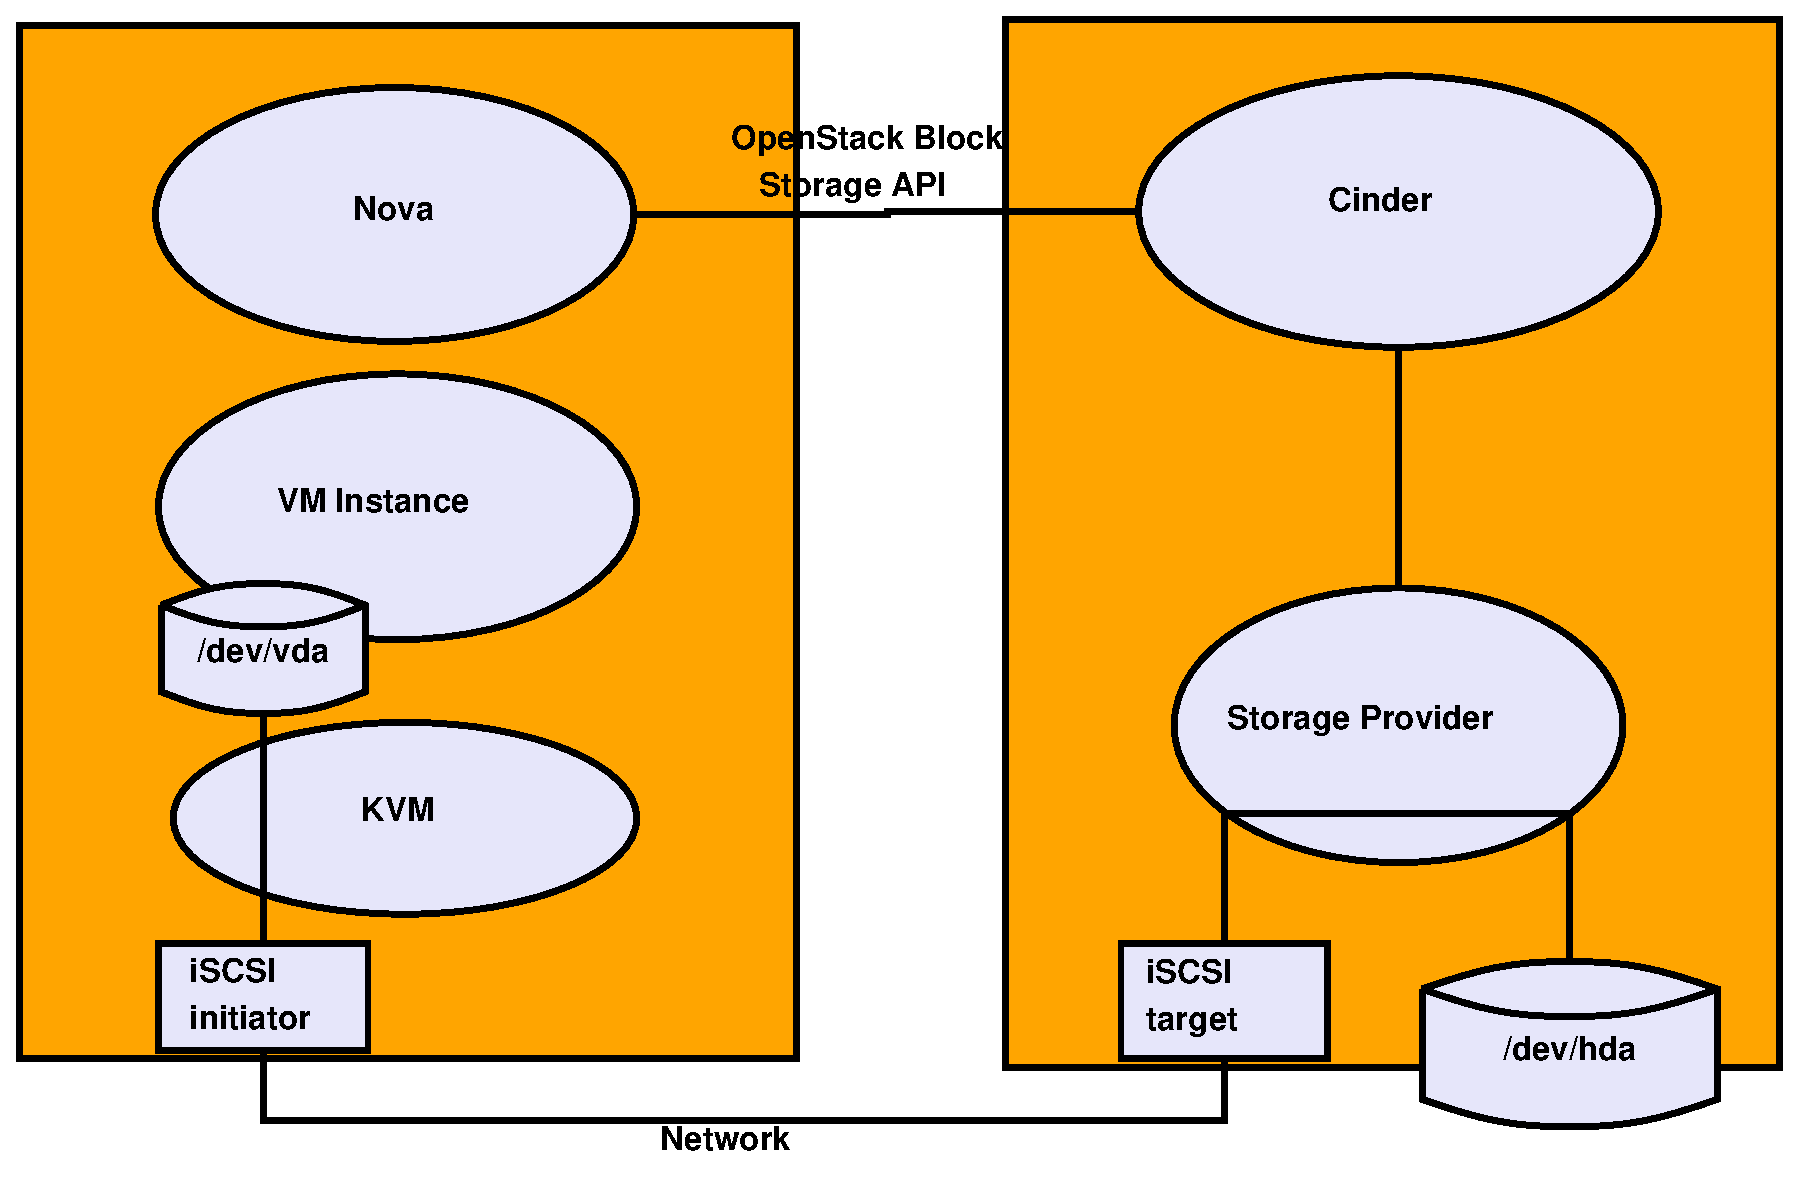
\includegraphics[scale=0.30]{cinder.eps}}

\end{frame}

\begin{frame}{Cinder: components interaction 2/3}

Interaction example:

\begin{itemize}
\item nova calles cinder-api with connection information (hostname, iSCSI initiator name, etc),
\item cinder-api writes the information in the DB and passes the message to cinder-scheduler,
\item cinder-scheduler chooses the back-end to be used for the volume provisioning and calles cinder-volume,
\item cinder-volume accesses the storage back-end using its driver passing the conf. parameters,
\end{itemize}

\end{frame}

\begin{frame}{Cinder: components interaction 3/3}

Interaction example:

\begin{itemize}
\item the storage back-end allows the connection and allocates the storage space,
\item cinder-volume returns then the connection information to nova,
\item nova creates the connections using the given parameteres and passes the volume device/file to the hypervisor.
\itme the hypervisor attaches the volume to the VM.
\end{itemize}

\end{frame}

\begin{frame}{Notes and Remarks}

\begin{itemize}
\item Logs directory is: \texttt{/var/log/cinder}
\item Files you are going to edit often:
      \begin{itemize}
        \item cinder-api conf. file is: \texttt{/etc/cinder/cinder-api.conf}
        \item cinder-volume conf. file is: \texttt{/etc/cinder/cinder-volume.conf}
      \end{itemize}
\item We will see everything in more detail during the tutorial.
\end{itemize}

\end{frame}

\begin{frame}{Useful Links}

\begin{itemize}
\item {\color{blue}\href{http://docs.openstack.org/icehouse/install-guide/install/apt/content/ch\_cinder.html}{Configure Cinder}}
\item {\color{blue}\href{https://wiki.openstack.org/wiki/Cinder}{Cinder Project Documentation}}
\end{itemize}

\end{frame}



\end{document}

%%% Local Variables:
%%% mode: latex
%%% TeX-master: t
%%% End:
